\chapter{数据:模拟暗物质晕表、SDSS观测数据及其模拟光锥星系表}
\label{cha:data}

\section{引言}

在使用BOSS/SDSS-III CMASS样本前,需要在很大的空间里用许多组星系表或暗物质晕表研究巨洞的统计性质。我们用基于微扰论的近似方法~\cite{Kitaura2014,Kitaura2015}(The PerturbAtion Theory Catalogue generator of Halo and galaxY,\textsc{PATCHY})生成了100组具有相同宇宙学模型的模拟暗物质晕表(mock catalogues)。这100组模拟暗物质晕表唯一的区别是生成它们各自初始密度场时随机数生成器使用了不同的种子(seeds),其他参数完全一样。这100组模拟暗物质晕表在后文被称作完整的模拟暗物质晕表(Complete halo mock catalogues)。

\textsc{PATCHY}使用BigMultiDark N-body simulations~\cite{Klypin2014}作为基准对参数进行标定,其宇宙学参数与Planck $\Lambda$CDM的宇宙学一致:$\Omega_{\rm M} = 0.307115$、$\Omega_b = 0.048206$、$\sigma_8 = 0.8288$、$n_s = 0.96$,哈勃参量为$H_0 \equiv 100\,h\,\mathrm{km}\,\mathrm{s}^{-1}\mathrm{Mpc}^{-1}$其中$h = 0.6777$。在边长为2.5\,$h^{-1}$ Gpc并具有周期性边界条件的立方体内,\textsc{PATCHY}将空间分为$960^3$个格点,网格的分辨率为2.6\,$h^{-1}$ Mpc,并通过augmented Lagrangian perturbation theory~\cite{Kitaura2013}(ALPT)来计算密度场。\textsc{PATCHY}细致的考虑了欧拉非线性偏袒(Eulerian non-linear bias)和随机偏袒(stochastic bias),并以此生成数密度为 $3.5\times10^{-4}\,h^3\,\mathrm{Mpc}^{-3}$的暗物质晕表。这个数密度与BOSS CMASS LRG样本在平均红移$z \simeq 0.56$处的平均数密度相同。

因为\textsc{PATCHY}是基于微扰论生成的暗物质晕表,这些暗物质晕表相对于用宇宙学大尺度结构N体数值模拟产生的模拟暗物质晕表不够准确,但是在统计性质上(两点和三点统计性质)可以十分接近~\cite{Chuang2015,Zhaocheng2015},在后文中如果不特别强调是由N体数值模拟产生的模拟暗物质晕表,模拟暗物质晕表都是指基于\textsc{PATCHY}生成的模拟暗物质晕表。我们使用这些模拟暗物质晕表研究巨洞的平均2PCF和估算协方差矩阵。

之后使用了BOSS/SDSS-III CMASS样本的DR11
%和DR12两部分
观测数据和相应的1024组与观测数据具有相似空间分布与统计性质的模拟星系表。这些模拟星系表也是用\textsc{PATCHY}生成的,经过Halo Abundance Matching~\cite{Rodriguez-Torres2016}(HAM)将模拟暗物质晕表转换成模拟星系表,把不同红移处的星系模拟星系表拼接起来并使具有光锥一样的几何形状,在后文被称作\textsc{PATCHY}光锥模拟星系表或模拟光锥星系表。本章详细介绍了这几组不同的模拟暗物质晕表、模拟光锥星系表和观测数据。

\section{完整的模拟暗物质晕表}
\label{sec:datacomple}

我们用\textsc{PATCHY}在边长为2.5\,$h^{-1}$Gpc并具有周期性边界条件的立方体内生成了100组模拟暗物质晕表。这100组完整的模拟暗物质晕表具有相同宇宙学模型,唯一的区别是生成各自初始密度场时随机数生成器使用了不同的种子。这些模拟暗物质晕表记录了暗物质晕在共动距离($h^{-1}$ Mpc)下的位置坐标($x_1$,$x_2$,$x_3$)和对应方向的速度($v_1$,$v_2$,$v_3$),数密度为$3.5\times10^{-4}\,h^3\,\mathrm{Mpc}^{-3}$,且所有暗物质晕都在红移$z = 0.5618$处。这些模拟暗物质晕表内记录的位置是暗物质晕在空间的真实位置,所以这部分数据被称为实空间模拟暗物质晕表(real space mock halo catalogues)。

假设观测者在$x_3$方向的无穷远处观测实空间完整模拟暗物质晕表内所记录的暗物质晕的红移和方向,暗物质晕的在$x_3$方向的本动速度会使其被观测到的红移发生变化,从而使其位置相对真实位置也发生一定程度的偏移。
这个因本动速度影响而使被观测天体位置相对真实位置发生偏移的现象叫做红移畸变效应(redshift space distortion,RSD)。
考虑RSD效应的完整模拟暗物质晕表的位置信息,与在无穷远处的观测者通过观测到的红移而转换成的位置信息相同,因此考虑RSD效应的完整模拟暗物质晕表被称作红移空间模拟暗物质晕表(redshift space mock halo catalogues)。

\begin{figure}
\centering
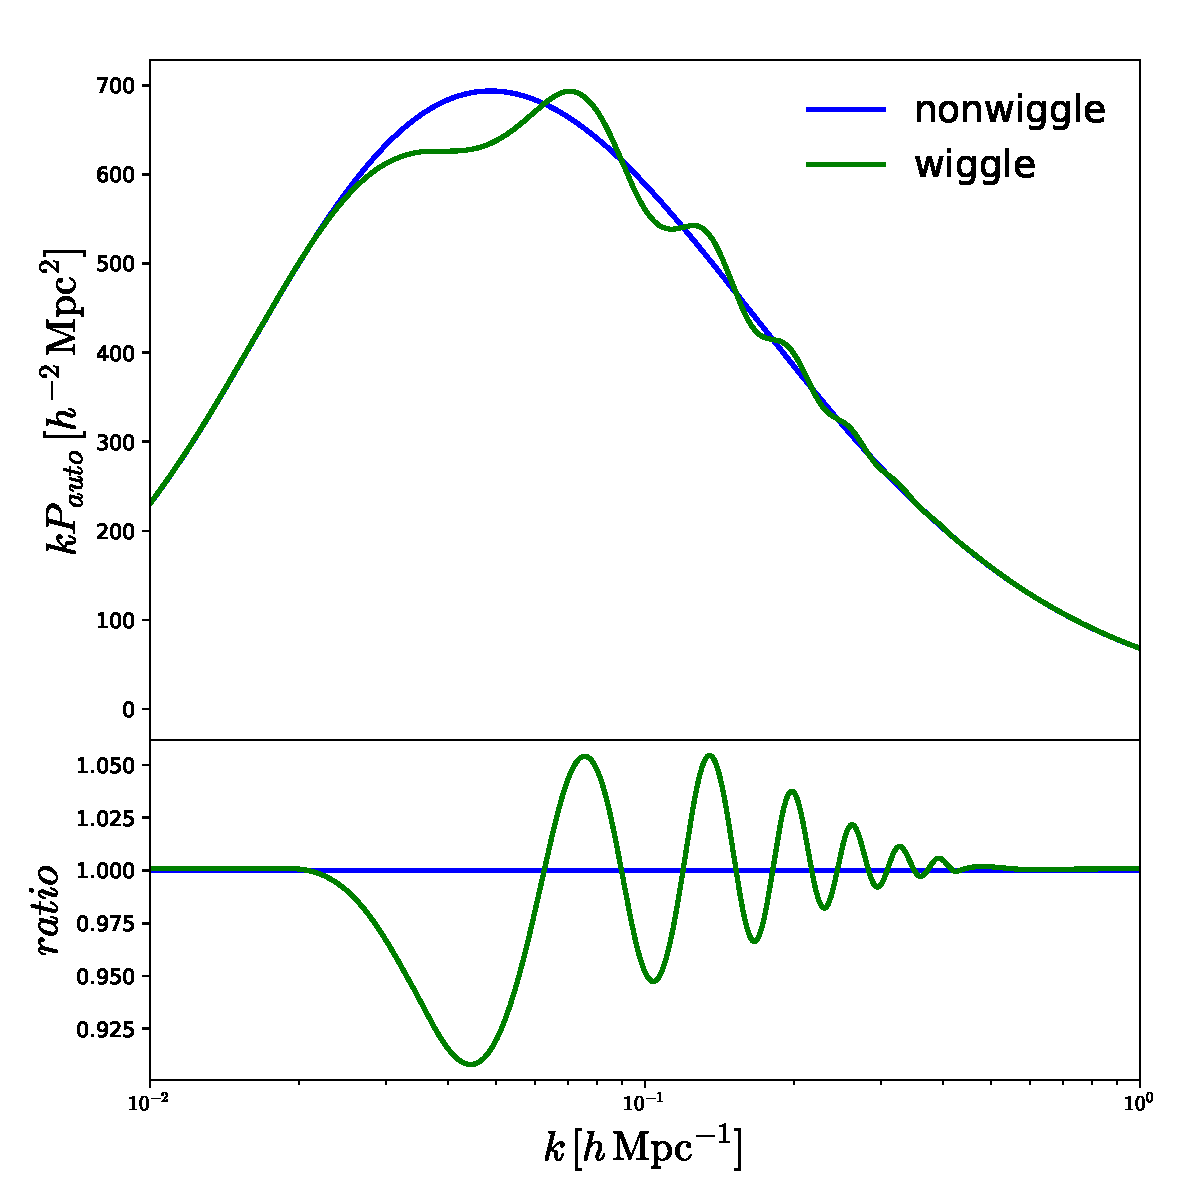
\includegraphics[width=.9\textwidth]{pk_ratio}
\caption{\textsc{PATCHY}所使用的两个初始物质功率谱,绿色实线是用Planck $\Lambda$CDM的宇宙学通过CAMB计算得到的有声学振荡的物质密度功率(wiggle),对绿色实线做平滑得到蓝色实线,也就是没有声学振荡的物质密度功率谱(nonwiggle)。上图画出来两个功率谱的形状,为了更清晰的表现两者的形状图中画的是$k P_{auto}$,下图展示了两个功率谱的比值。}
\label{fig:pkratio}
\end{figure}

\section{无BAO的完整的模拟暗物质晕表}
\label{sec:datanw}

用\textsc{PATCHY}在边长为2.5\,$h^{-1}$Gpc并具有周期性边界条件的立方体内生成了100组模拟暗物质晕表,生成这些模拟暗物质晕表的初始密度场的功率谱中没有声学振荡的成分,其他条件与实空间的100组完整模拟暗物质晕表完全相同。图~\ref{fig:pkratio} 展示了这些没有声学振荡的初始密度功率谱与前面实空间完整模拟暗物质晕表的初始密度功率谱。因为声学振荡在初始密度功率谱的特征就是图~\ref{fig:pkratio} 中下半部分所示的一系列振荡,通过对有声学振荡初始密度功率谱做平滑可以得到没有声学振荡的初始密度功率谱。

\section{\textsc{PATCHY}光锥模拟星系表}
\label{sec:lightcone}

利用观测数据能得到一个测量结果,有两大类方法可以去估算测量结果的误差。一种是将整个巡天分成几份,把每一份当成一个独立的观测,然后通过刀切法复采样(jackknife resampling)或自举复采样(bootstrap resampling)来估算误差。这种方法虽然曾经被使用过~\cite{Norberg2009},但是并不能很好的考虑系统误差的影响,不容易帮助人们研究结果背后的物理。另外体积变小后,对于比子样本体积更大的尺度上的误差估算会非常不可靠,这一点对于研究BAO尤为致命。另一种方法是用许多组宇宙大尺度结构数值模拟的数据来估算观测结果的误差,这种方法估算的误差更加可靠。使用N体数值模拟可以非常精确的再现宇宙大尺度结构,但是这种方式需要非常大的计算量,不可能批量生成上千组结果。而\textsc{PATCHY}可以比较精确的再现宇宙大尺度结构,其两点、三点统计性质与N体数值模拟的结果相差非常小,同时其对计算量的需求远远小于N体数值模拟。所以BOSS最后两次发布的数据都采用了\textsc{PATCHY}生成的光锥模拟星系表来估算观测结果的误差。

生成可靠的\textsc{PATCHY}光锥模拟星系表以估算观测结果的误差需要进行以下几步处理:
\begin{description}
\item[1.] 使用N体数值模拟(BigMultiDark Simulations~\cite{Klypin2014})在一系列不同红移处,生成可以精确呈现暗物质晕内部子结构的暗物质晕表。在不同的红移处,选用适当的参数通过HAM把模拟暗物质晕表转化成模拟星系表~\cite{Rodriguez-Torres2016}。
\item[2.] 在不同红移处,分别调整\textsc{PATCHY}的参数,使其生成的暗物质晕模拟暗物质晕表与所在红移处的模拟星系表具有相同的两点和三点成团性。
\item[3.] 用HADRON~\cite{Zhaocheng2015}(Halo mAss Distribution ReconstructiON)计算\textsc{PATCHY}生成的每一个暗物质晕的恒星质量。
\item[4.] 用SUGAR~\cite{Rodriguez-Torres2016}(The SUrvey GenerAtoR)将不同红移处的\textsc{PATCHY}模拟星系表拼接成光锥模拟星系表,并使其与观测数据具有一样的几何形状、巡天区域和选择效应,并在整个空间与观测数据具有相同的数密度分布。
\end{description}

BOSS DR11一共有1024个\textsc{PATCHY}光锥模拟星系表,BOSS DR12有2048个\textsc{PATCHY}光锥模拟星系表,这些数据被用于后续的相应研究。图~\ref{fig:pie} 展示了在Southern Galactic Cap(SGC)和Northern Galactic Cap(NGC),\textsc{PATCHY}光锥模拟星系表很好的再现了BOSS DR12在空间的分布。

\begin{figure}
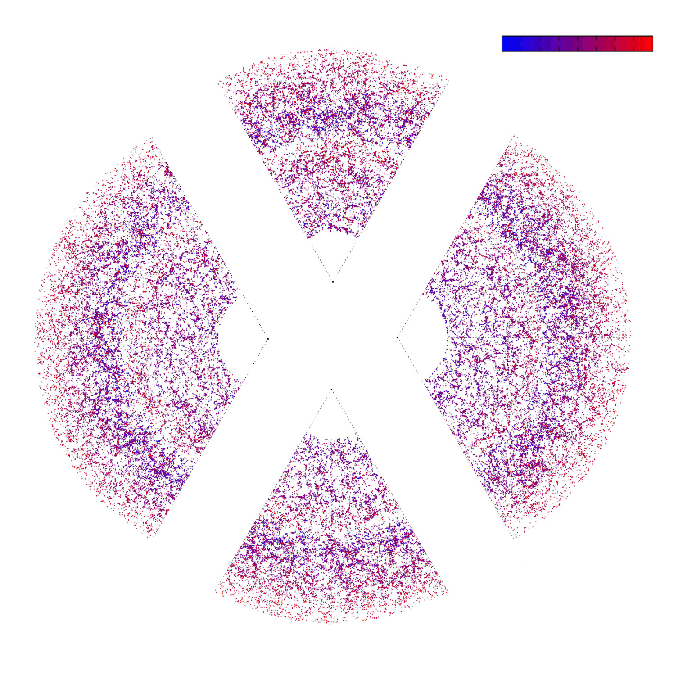
\includegraphics[width=15.cm]{pie}
\put(-380,390){\rotatebox[]{0}{BOSS DR12}}
\put(-125,45){\rotatebox[]{0}{MULTIDARK}}
\put(-125,30){\rotatebox[]{0}{PATCHY MOCKS DR12}}
\put(-20,210){\rotatebox[]{-90}{180$^{\rm o}$}}
\put(-417,210){\rotatebox[]{90}{180$^{\rm o}$}}
\put(-10,210){\rotatebox[]{-90}{\text{Northern Galactic Cap}}}
\put(-427,210){\rotatebox[]{90}{\text{Northern Galactic Cap}}}
\put(-40,290){\rotatebox[]{-90}{210$^{\rm o}$}}
\put(-397,290){\rotatebox[]{90}{150$^{\rm o}$}}
\put(-100,350){\rotatebox[]{-90}{240$^{\rm o}$}}
\put(-337,350){\rotatebox[]{90}{120$^{\rm o}$}}
\put(-40,130){\rotatebox[]{-90}{150$^{\rm o}$}}
\put(-397,130){\rotatebox[]{90}{210$^{\rm o}$}}
\put(-100,70){\rotatebox[]{-90}{120$^{\rm o}$}}
\put(-337,70){\rotatebox[]{90}{240$^{\rm o}$}}
\put(-145,380){\rotatebox[]{0}{330$^{\rm o}$}}
\put(-297,380){\rotatebox[]{0}{30$^{\rm o}$}}
\put(-145,40){\rotatebox[]{0}{30$^{\rm o}$}}
\put(-297,40){\rotatebox[]{0}{330$^{\rm o}$}}
\put(-255,410){\rotatebox[]{0}{\text{Southern Galactic Cap}}}
\put(-220,400){\rotatebox[]{0}{0$^{\rm o}$}}
\put(-220,23){\rotatebox[]{0}{0$^{\rm o}$}}
\put(-255,13){\rotatebox[]{0}{\text{Southern Galactic Cap}}}
\put(-192,280){\rotatebox[]{0}{2.7}}
\put(-252,280){\rotatebox[]{0}{0.2}}
\put(-172,315){\rotatebox[]{0}{5.1}}
\put(-272,315){\rotatebox[]{0}{0.4}}
\put(-152,350){\rotatebox[]{0}{7.3}}
\put(-292,350){\rotatebox[]{0}{0.6}}
%
\put(-195,300){\rotatebox[]{60}{\text{lookback time in billions of years}}}
%
\put(-280,300){\rotatebox[]{-60}{\text{redshift}}}
%
\put(-260,233){\rotatebox[]{-58}{\Huge$\leftharpoondown$}} %longleftarrow$}}
\put(-190,183){\rotatebox[]{-238}{\Huge$\leftharpoondown$}} %longleftarrow$}}
\put(-275,220){\rotatebox[]{0}{\text{OBSERVATIONS}}}
\put(-225,200){\rotatebox[]{0}{\text{THEORY/MODEL}}}
\put(-192,145){\rotatebox[]{0}{2.7}}
\put(-252,145){\rotatebox[]{0}{0.2}}
\put(-172,110){\rotatebox[]{0}{5.1}}
\put(-272,110){\rotatebox[]{0}{0.4}}
\put(-152,75){\rotatebox[]{0}{7.3}}
\put(-292,75){\rotatebox[]{0}{0.6}}
\put(-73,410){\rotatebox[]{0}{\text{log M$_*$}}}
\put(-115,388){\rotatebox[]{0}{\tiny\text{10.9}}}
\put(-90,388){\rotatebox[]{0}{\tiny\text{11.1}}}
\put(-67,388){\rotatebox[]{0}{\tiny\text{11.3}}}
\put(-43,388){\rotatebox[]{0}{\tiny\text{11.5}}}
\put(-20,388){\rotatebox[]{0}{\tiny\text{12.0$<$}}}
\caption{ BOSS DR12 观测数据(左上部分)和\textsc{PATCHY光锥模拟星系表}(\textsc{MULTIDARK PATCHY MOCKS DR12},右下部分)在空间中的分布。(文献 ~\inlinecite{Kitaura2016}中的Figure 2)}
\label{fig:pie}
\end{figure}

\begin{figure}
\centering
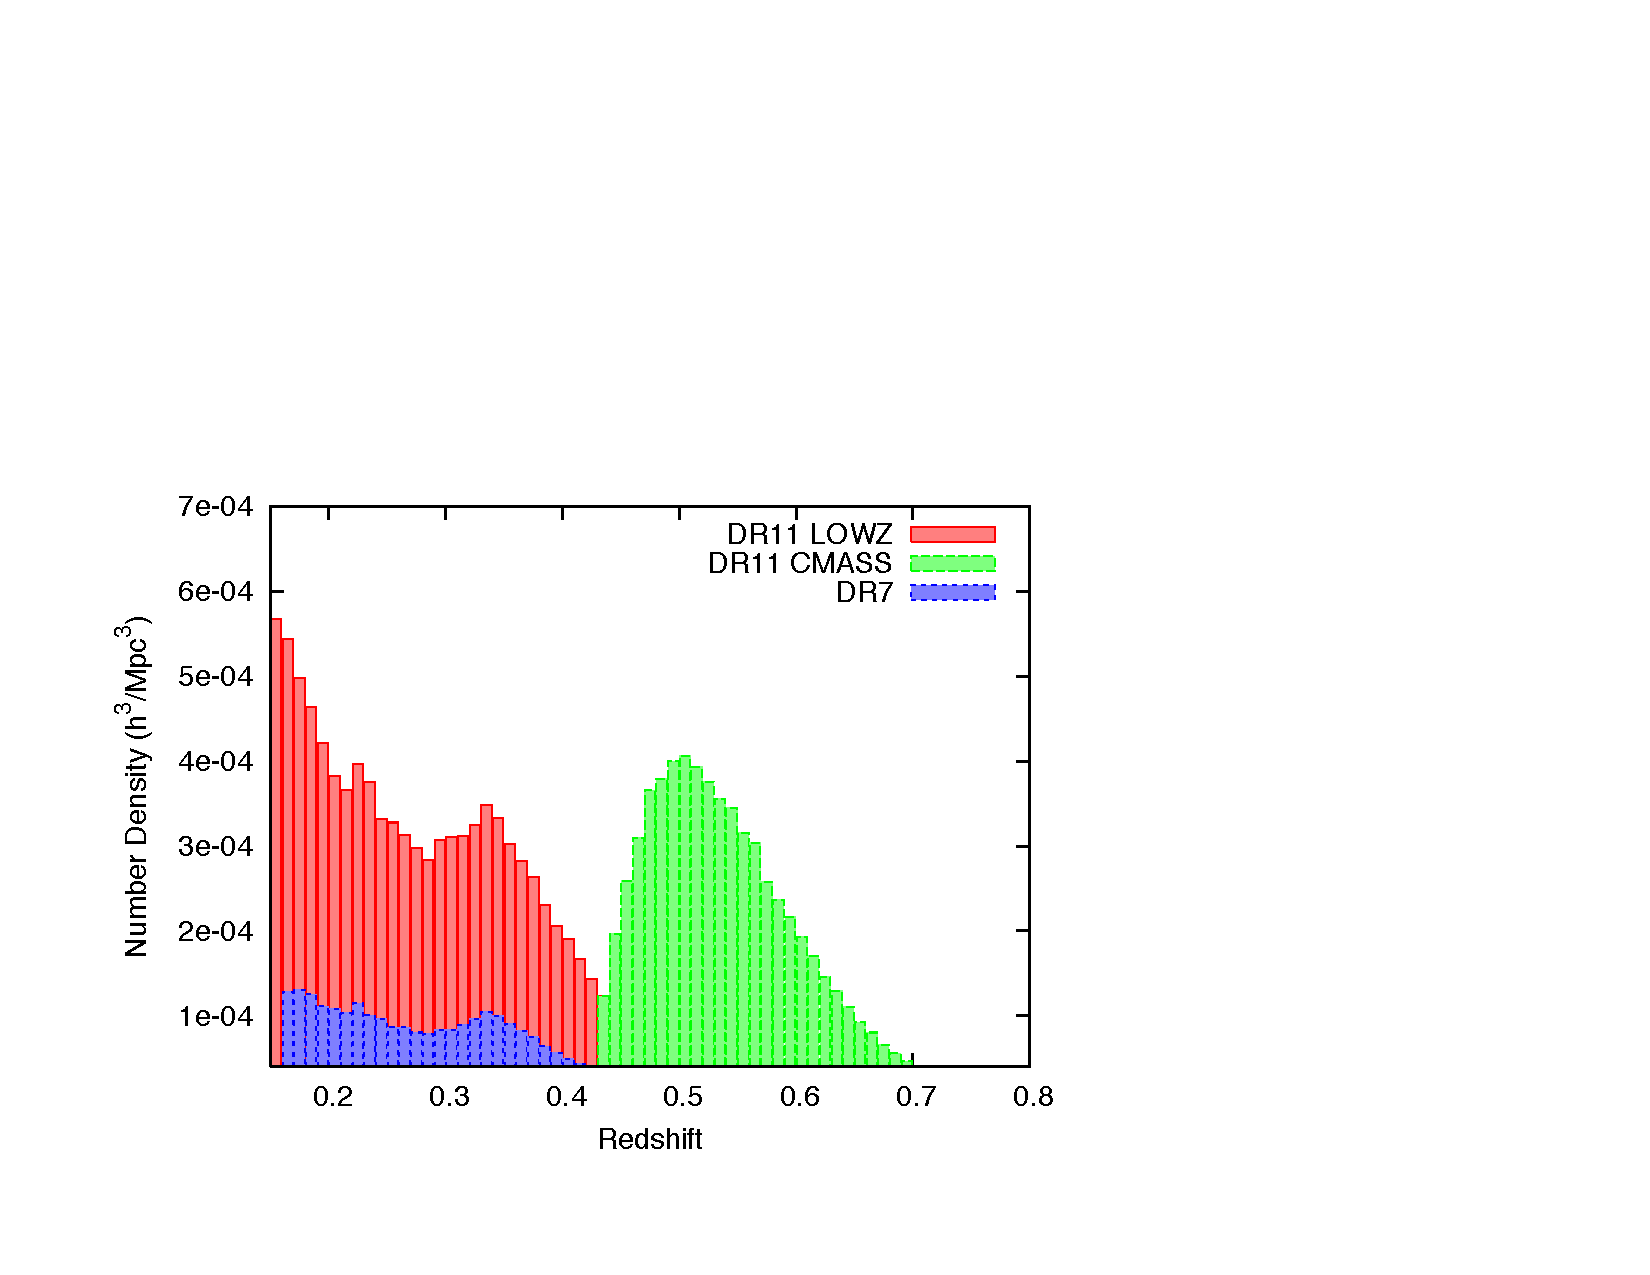
\includegraphics[width=.9\textwidth]{Anderson2014_figure1_dNdzhist}
\caption{BOSS/SDSS DR11 样本中LOWZ(红色)和CMASS(绿色)的星系数密度随红移的分布。蓝色柱状图是SDSS-II DR7的星系数密度随红移的分布~\cite{Abazajian2009DR7}。(文献 ~\inlinecite{Anderson2014441} 中的Figure 1)}
\label{fig:AndersonFig1}
\end{figure}

\section{BOSS/SDSS-III CMASS DR11星系表}

BOSS~\cite{Eisenstein:2011sa, Bolton:2012hz, Dawson2013}是SDSS-III的重要组成部分,观测使用的是位于新墨西哥州(New Mexico)的阿帕奇天文台(Apache Point Observatory)的2.5米斯隆望远镜(Sloan Telescope)~\cite{Gunn2006}。BOSS使用了相比SDSS I/II升级后的光谱仪,可以得到波长范围3600-10000\r{A}内分辨率为1500-2600\r{A}的光谱~\cite{Smee2013}。计划在10000平方度的天区内,LOWZ和CMASS两个红移区间,获得135万个星系的光谱和红移(图~\ref{fig:AndersonFig1})。这些星系是通过SDSS DR8~\cite{Aihara2011}的图像观测筛选出来的LRG。我们的工作中只使用了CMASS样本。从SDSS DR8中筛选CMASS目标LRG的条件为
\begin{eqnarray}
 17.5 < i_{\rm cmod}  < 19.9\\
r_{\rm mod} - i_{\rm mod}  < 2 \\
d_{\perp} > 0.55 \label{eq:hcut}\\
i_{\rm fib2} < 21.5\\
i_{\rm cmod}  < 19.86 + 1.6(d_{\perp} - 0.8) \label{eq:slide}
\end{eqnarray}
其中$i$和$r$是相应波段的星等,$i_{\rm fib2}$是$i$波段在2角秒孔径的星等,下标“mod”指$r$波段德沃古勒(DeVaucouleurs)和指数轮廓(exponential profile)的最佳拟合值~\cite{Stoughton2002},下标“cmod”指段德沃古勒和指数轮廓线性组合的最佳拟合值~\cite{Abazajian2004},$d_{\perp}$定义为
\begin{equation}
d_{\perp} = r_{\rm mod} - i_{\rm mod} - (g_{\rm mod} - r_{\rm mod})/8.0
\label{eq:dp}
\end{equation}
将星系与恒星区分开的条件是
\begin{eqnarray}
i_{\rm psf} - i_{\rm mod} > 0.2 + 0.2(20.0-i_{\rm mod})  \label{eq:sgsep1}\\
z_{\rm psf}-z_{\rm mod} > 9.125 -0.46\,z_{\rm mod} \label{eq:sgsep2},
\end{eqnarray}
其中下标“psf”指点扩散函数(point spread function)。

CMASS的星系分布在红移$0.43 < z < 0.7$的范围内,星系数密度在 $z \approx 0.5$达到峰值(图~\ref{fig:AndersonFig1})。对于BOSS CMASS DR11观测数据和光锥模拟星系表的研究,我们只使用了红移$0.45 < z < 0.65$内的数据。图~\ref{fig:footprints}展示了DR11所覆盖的天区。

BOSS的样本中存在一些系统性偏差,比如有些星系不能测量红移(redshift failure),或者因为获取星系光谱时,相邻两根光纤的最近距离不能小于$55^{\prime\prime}$从而造成一些星系无法被观测到(fiber collision)。而星系成团性分析的结果会严重受到这些问题影响。通过文献 ~\inlinecite{Ross2012}中提出的方法,给每个星系不同的权重可以在一定程度上减小系统性偏差对星系成团性的影响~\cite{Ross2012,Chuang2016}。每个星系的权重是
\begin{equation}
w_g = w_{star} w_{see} (w_{zf} + w_{cp} - 1)
\label{EQ:weight}
\end{equation}
其中$w_{zf}$是测量红移失败的权重,$w_{cp}$是两个星系离的很近的权重(the close pair weight),$w_{star}$是用来处理星系数密度与恒星数密度系统性关系的权重,$w_{see}$是修正视宁度(seeing)的权重。$w_{zf}$和$w_{cp}$对CMASS样本的影响很小~\cite{Ross2012},所以在光锥模拟星系表中没有考虑这两个权重所对应的效应。DR11 CMASS样本使用这个方法计算出了每个星系的权重~\cite{Anderson2014441},计算观测星系2PCF时使用了这些权重。图~\ref{fig:CMASSpkxi}中是BOSS CMASS DR11观测样本星系的2PCF和功率谱。

\begin{figure}
\centering
\resizebox{\textwidth}{!}{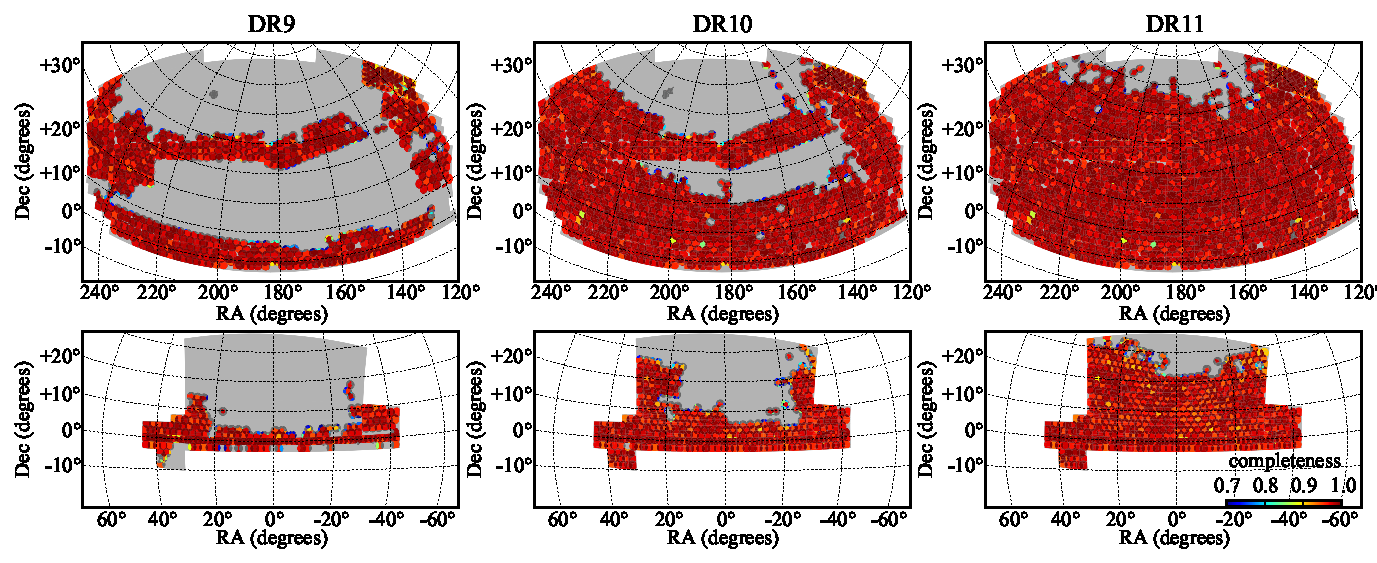
\includegraphics{BOSS_CMASS_footprint_comparison1}}
\caption{ 从BOSS DR9到DR11巡天观测所覆盖的天区。上半部分是NGC方向的结果,下半部分是SGC方向的结果。不同颜色表示了光谱测量的完成度。灰色区域是BOSS计划观测但是尚未观测的天区。DR9、DR10和DR11所覆盖的天区面积分别为3275、6161和8377平方度。(文献 ~\inlinecite{Anderson2014441} 中的Figure 2)}
\label{fig:footprints}
\end{figure}

\begin{figure}
\centering
\resizebox{0.8\textwidth}{!}{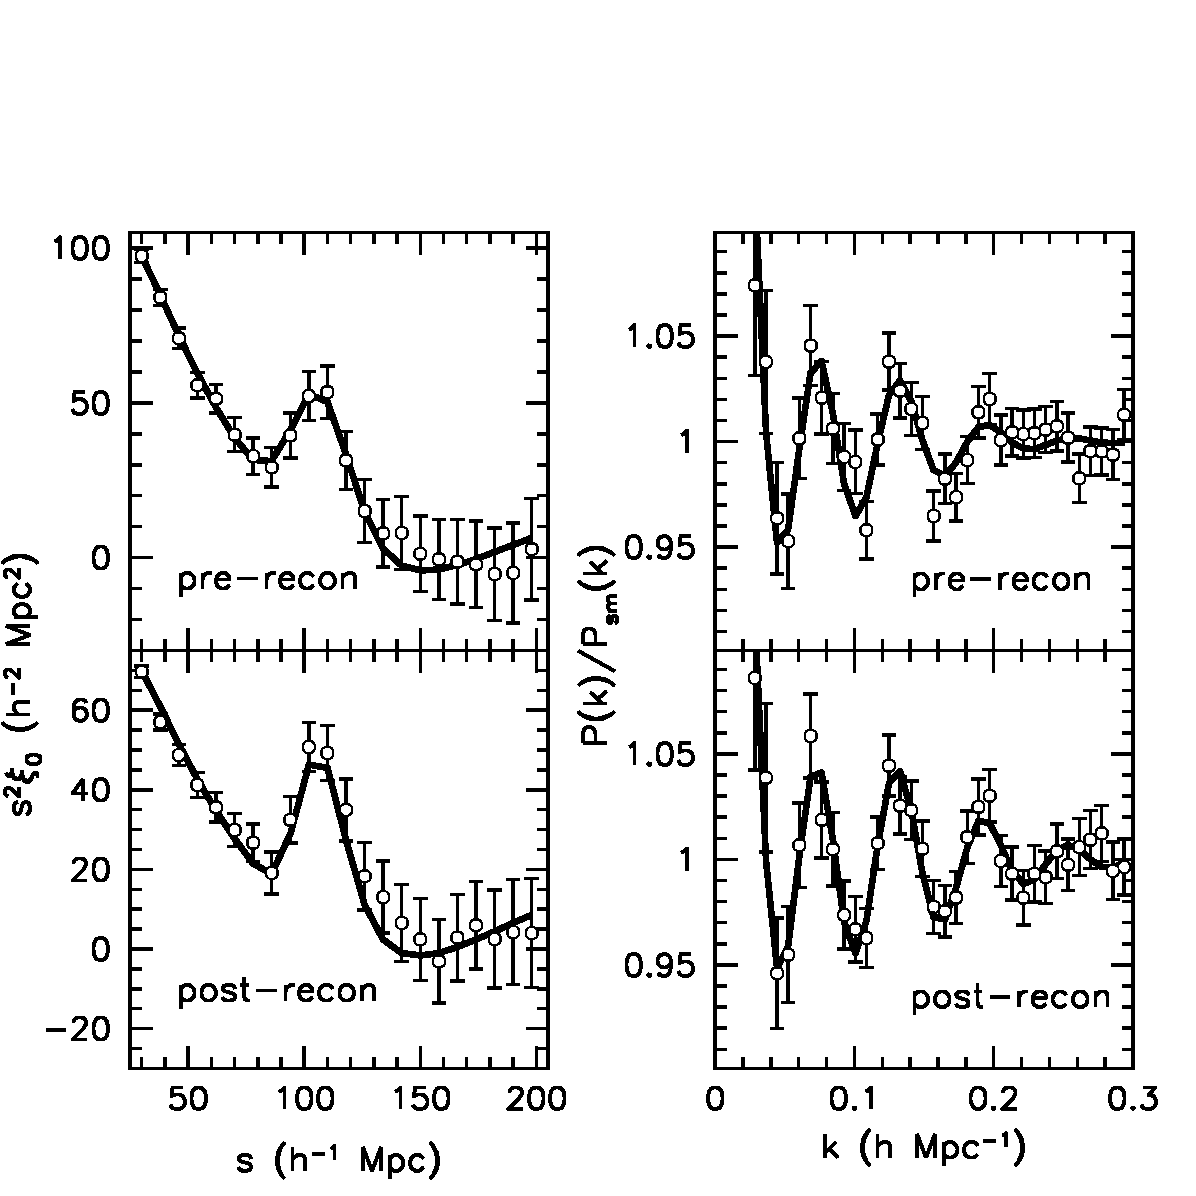
\includegraphics{aard2pt4pan_CMASS.pdf}}
\caption{DR11 CMASS 样本的2PCF$\xi(s)$(左半部分),和功率谱$P(k)$(右半部分)。上半部分是没有经过BAO信号重构的结果,下半部分是经过BAO信号重构的结果。实线是每个情况的最佳拟合。BAO信号重构之后的$\xi(s)$和$P(k)$中,BAO信号的显著性都得到增强。(文献 ~\inlinecite{Anderson2014441} 中的Figure 11)}
\label{fig:CMASSpkxi}
\end{figure}

%\section{BOSS/SDSS-III CMASS DR12星系表}